%% ============================================================
%% Supplementary Material -- skeleton (revised)
%% Companion to: "Porous polyimide/hexagonal boron nitride films by
%% non-solvent induced phase separation: a three-phase Lewis--Nielsen
%% description of dielectric and thermal properties"
%% Compile with pdfLaTeX. Section numbering uses the S-prefix.
%% Orange \hl{} marks = content to be completed by the authors.
%% ============================================================
\documentclass[10pt,a4paper]{article}
\usepackage[margin=2.4cm]{geometry}
\usepackage[T1]{fontenc}
\usepackage[utf8]{inputenc}
\usepackage{graphicx}
\usepackage{amsmath}
\usepackage{siunitx}
\usepackage{booktabs}
\usepackage{xcolor}
\usepackage{setspace}
\usepackage[font=footnotesize]{caption}
\newcommand{\hl}[1]{\colorbox{orange}{\parbox{0.93\linewidth}{#1}}}
\usepackage[colorlinks=true,linkcolor=blue,citecolor=blue]{hyperref}
\graphicspath{{figures/}}

\sisetup{per-mode=power}

% S-prefixed numbering
\renewcommand{\thesection}{S\arabic{section}}
\renewcommand{\thefigure}{S\arabic{figure}}
\renewcommand{\thetable}{S\arabic{table}}
\renewcommand{\theequation}{S\arabic{equation}}

\newcommand{\eps}{\ensuremath{\varepsilon_r}}
\newcommand{\lam}{\ensuremath{\lambda}}
\newcommand{\Apore}{\ensuremath{A_{\mathrm{pore}}}}
\newcommand{\ABN}{\ensuremath{A_{\mathrm{BN}}}}
\newcommand{\lamBN}{\ensuremath{\lambda_{\mathrm{BN,eff}}}}
\newcommand{\phimax}{\ensuremath{\phi_{\max}}}

\title{\bfseries Supplementary Material\\[4pt]
\large Porous polyimide/hexagonal boron nitride films by non-solvent induced phase separation: a three-phase Lewis--Nielsen description of dielectric and thermal properties}
\author{\hl{Author names --- to be completed}}
\date{}

\begin{document}
\setstretch{1.5}
\maketitle

%% ------------------------------------------------------------
\section{Supplementary model figures}
\label{si:modelfigs}

\subsection{Shape-factor sensitivity analysis}
\label{si:shapefactor}

Figure~\ref{fig:S1} examines the sensitivity of the three-phase Lewis--Nielsen
predictions to the h-BN shape factor $A$ over the range 0.3--6.0
(needle-like rods to aligned platelets), evaluated at the NP mean porosity
of 65.6\% with $\phimax = 0.60$ fixed. For the dielectric model
(Figure~\ref{fig:S1}a), all $A$ curves are nearly indistinguishable,
confirming that \eps{} is dominated by the pore term and that the fitted
dielectric \ABN{} is weakly determined. For the thermal model
(Figure~\ref{fig:S1}b), all $A = 0.3$--6.0 curves remain below the
experimental NP 70~wt\% value (0.16--0.18 vs.\
\SI{0.305}{\watt\per\meter\per\kelvin}), reinforcing that the 70~wt\%
enhancement is driven by proximity to maximum packing and incipient
particle contact rather than by any plausible single-particle shape factor.
Full discussion appears in Sections~3.2 and 4.6 of the main text.

\begin{figure}[htbp]
\centering
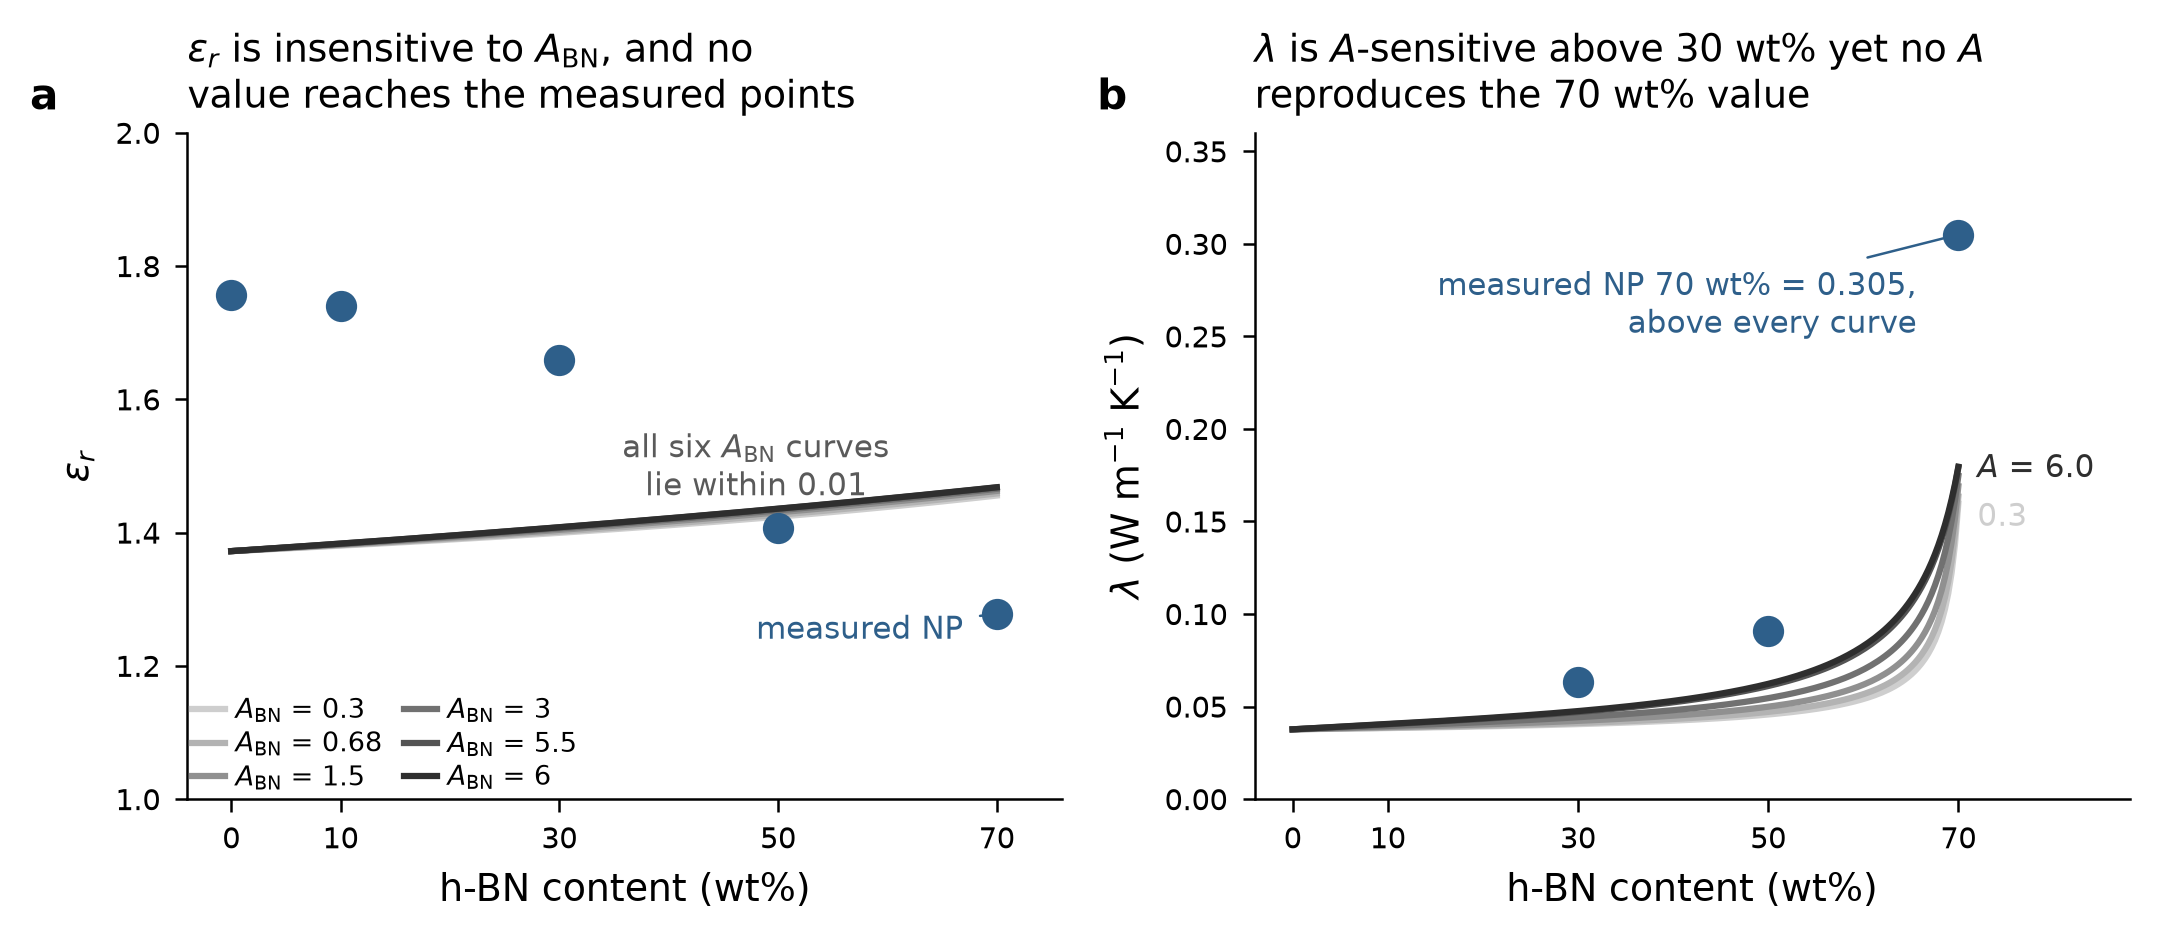
\includegraphics[width=0.95\linewidth]{FigS1.png}
\caption{Sensitivity of three-phase LN predictions to h-BN shape factor $A$
($A = 0.3$--6.0) for (a) dielectric constant and (b) thermal conductivity,
evaluated at the NP mean porosity of 65.6\% ($\phimax = 0.60$ fixed).
Symbols: measured NP data. In (a) all six curves lie within 0.01 of one
another, confirming that \eps{} is pore-dominated and \ABN{} weakly
determined; note also that no value of $A$ brings the curves onto the
measured points. In (b) the curves separate above 30~wt\% yet all remain
far below the measured NP 70~wt\% value of
\SI{0.305}{\watt\per\meter\per\kelvin}, so that enhancement cannot be
attributed to any plausible single-particle shape factor.}
\label{fig:S1}
\end{figure}

\subsection{Parity plot of the dielectric model}
\label{si:parity}
Figure~\ref{fig:S2} compares the three-phase LN prediction with the measured
dielectric constant for all ten films. The model RMSE (0.43 NP, 0.36 HP)
exceeds the standard deviation of the measured data (0.19 NP, 0.18 HP), so
the coefficient of determination is negative (Section~4.2 of the main
text); the numerical values are listed in Table~2 of the main text.

\begin{figure}[htbp]
\centering
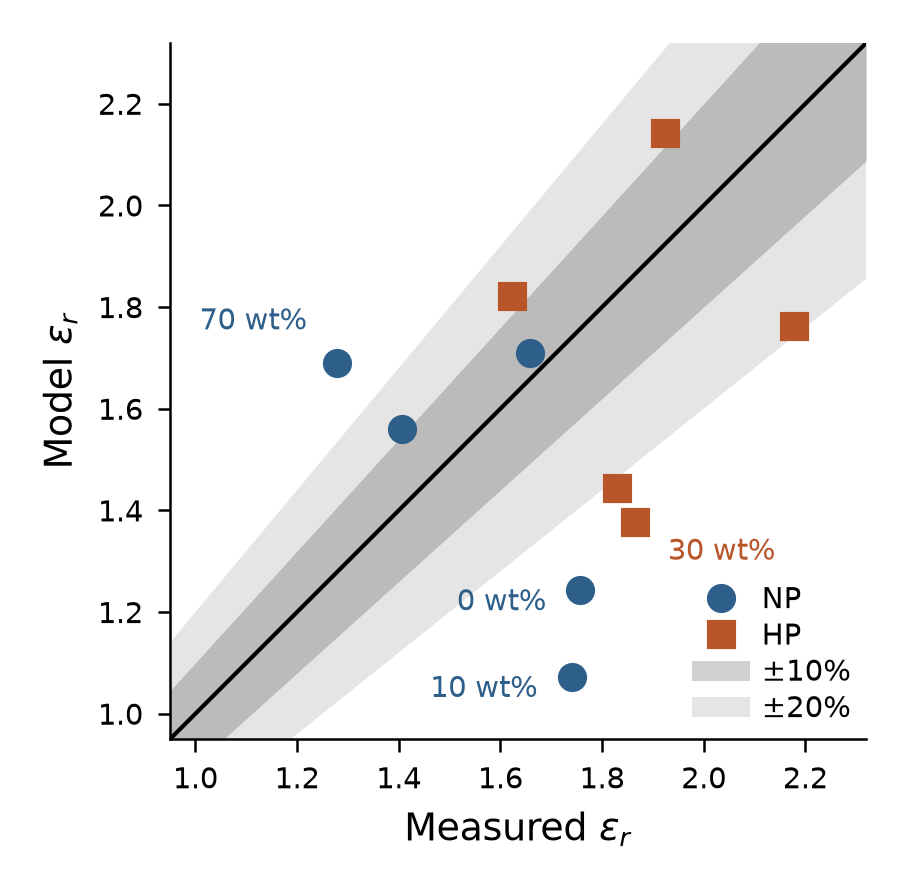
\includegraphics[width=0.55\linewidth]{FigS2_parity.png}
\caption{Parity plot of predicted vs.\ measured dielectric constant for all
ten films (three-phase LN model evaluated at each film's open porosity),
with $\pm$10\% and $\pm$20\% bands. Labels identify the compositions with
the largest residuals.}
\label{fig:S2}
\end{figure}

\subsection{Porosity sensitivity at fixed composition}
\label{si:porosity}
Figure~\ref{fig:S3} shows the calibrated \eps{} and \lam{} at fixed 50~wt\%
h-BN as porosity is varied. Both properties rise as porosity falls, so
porosity alone cannot decouple them; the same coupling is shown for every
composition by the loci of Figure~4c of the main text.

\begin{figure}[htbp]
\centering
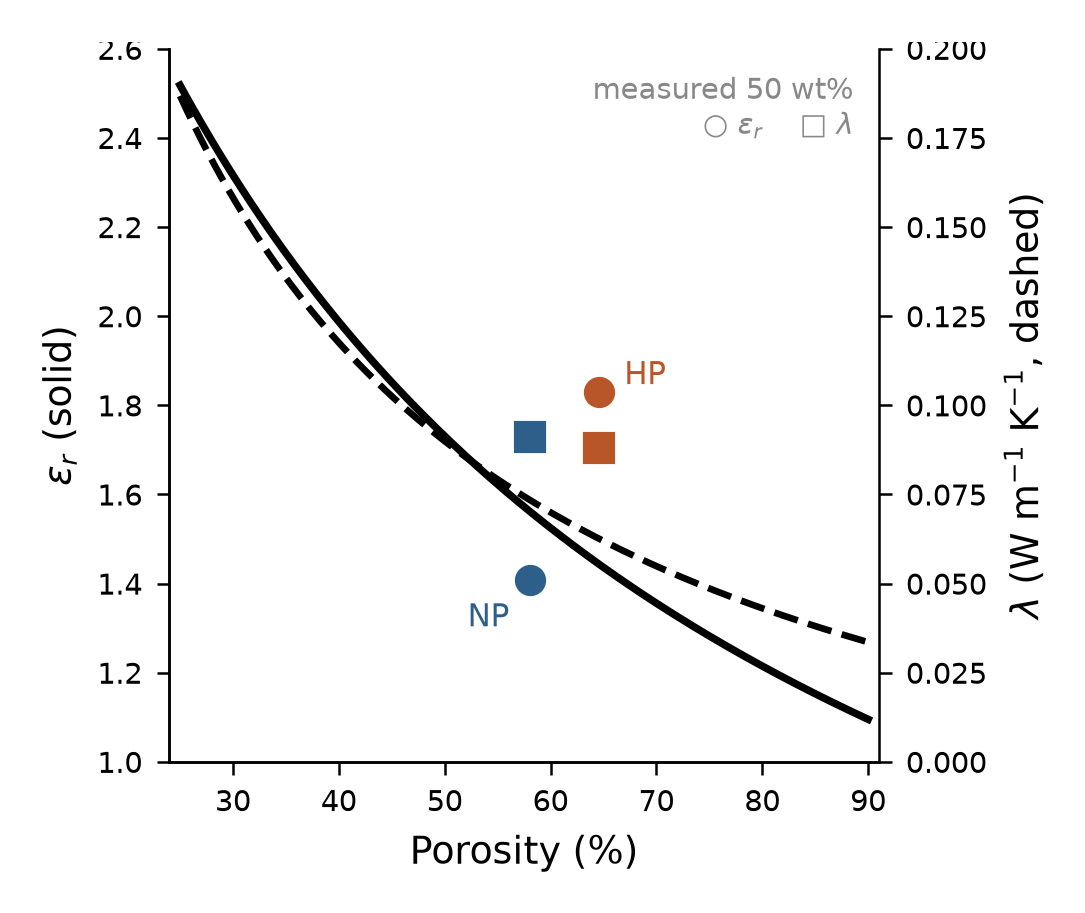
\includegraphics[width=0.6\linewidth]{FigS3_porosity_sensitivity.png}
\caption{Porosity sensitivity at fixed 50~wt\% h-BN: \eps{} (left axis,
solid) and \lam{} (right axis, dashed) from the calibrated three-phase LN
model. Circles and squares mark the measured NP and HP 50~wt\% films
(\eps{} and \lam, respectively).}
\label{fig:S3}
\end{figure}

\subsection{Feasible processing window}
\label{si:window}
Figure~\ref{fig:S4} shows the porosity range that satisfies each of the three
target specifications defined in Section~4.8 of the main text (Basic:
$\eps < 2.0$, $\lam > \SI{0.05}{\watt\per\meter\per\kelvin}$; Advanced:
$\eps < 1.8$, $\lam > \SI{0.08}{\watt\per\meter\per\kelvin}$; Future:
$\eps < 1.6$, $\lam > \SI{0.12}{\watt\per\meter\per\kelvin}$), derived from
the design maps of Figure~4a,b of the main text.

\begin{figure}[htbp]
\centering
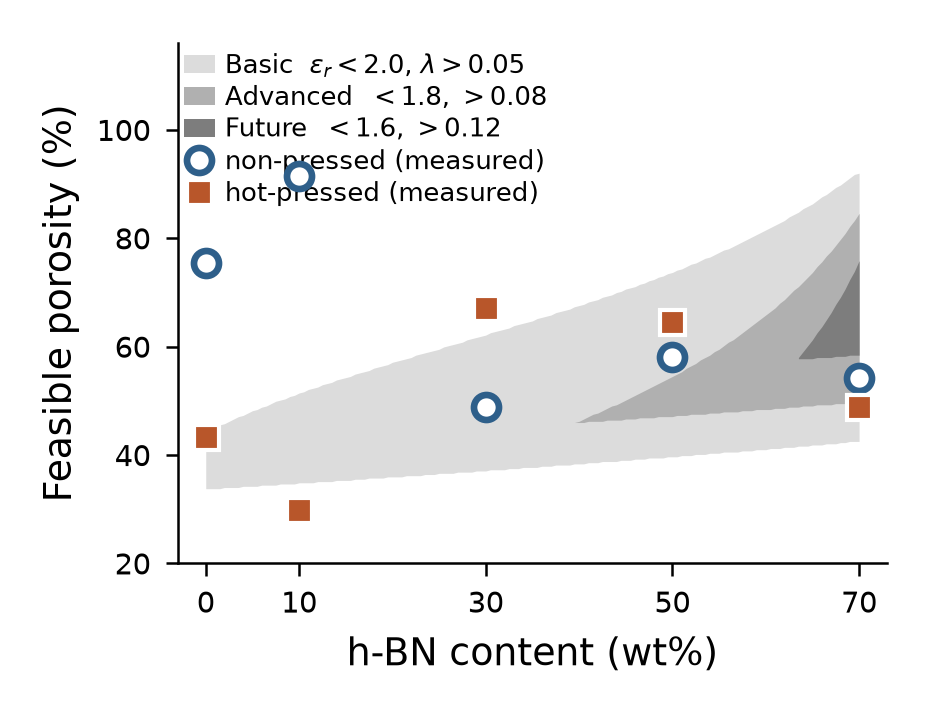
\includegraphics[width=0.6\linewidth]{FigS4_feasible_window.png}
\caption{Feasible processing window: the porosity range meeting each target
specification vs.\ h-BN content (nested shading, light to dark for
Basic$\to$Future); measured NP (open circles) and HP (filled squares)
states overlaid.}
\label{fig:S4}
\end{figure}

\subsection{Porosity that maximizes thermal conductivity under a dielectric ceiling}
\label{si:optimum}
Figure~\ref{fig:S5} shows, for each h-BN loading, the porosity that maximizes
\lam{} under a given \eps{} ceiling. The five composition curves stay within
10 percentage points of one another, so the porosity target is set almost
entirely by the dielectric ceiling while the achievable \lam{} at that
porosity is set by the loading (Section~4.8 of the main text).

\begin{figure}[htbp]
\centering
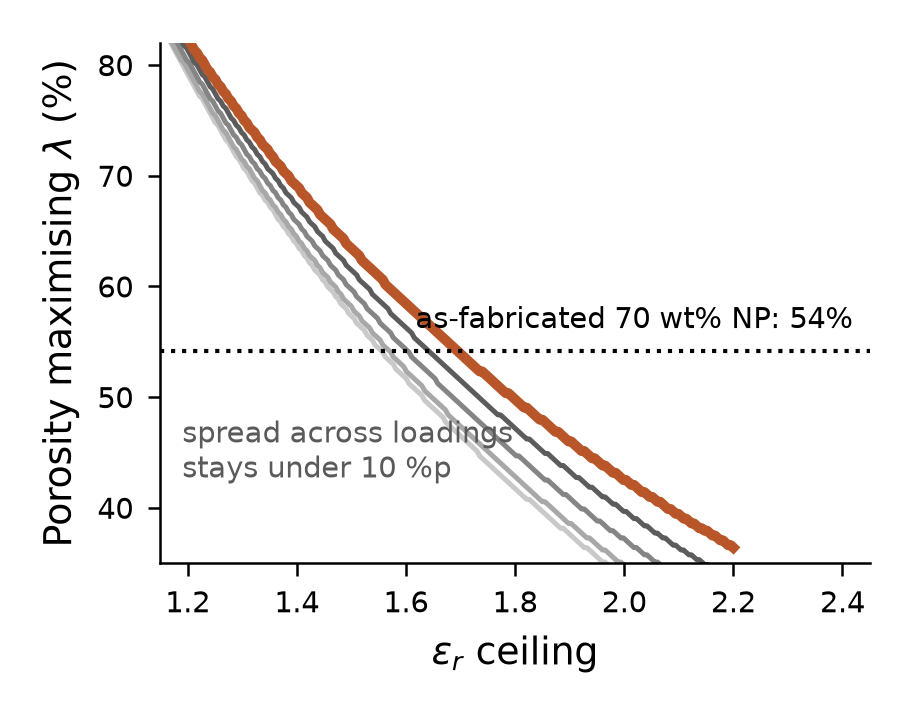
\includegraphics[width=0.6\linewidth]{FigS5_porosity_optimum.png}
\caption{Porosity that maximizes \lam{} under each \eps{} ceiling for
0--70~wt\% h-BN (light to dark grey, 0--50~wt\%; orange, 70~wt\%). The dotted
line marks the as-fabricated porosity of the 70~wt\% NP film (54\%).}
\label{fig:S5}
\end{figure}

%% ------------------------------------------------------------
\section{Additional materials characterization}
\label{si:characterization}

\subsection{Film photographs}
\begin{figure}[htbp]
\centering
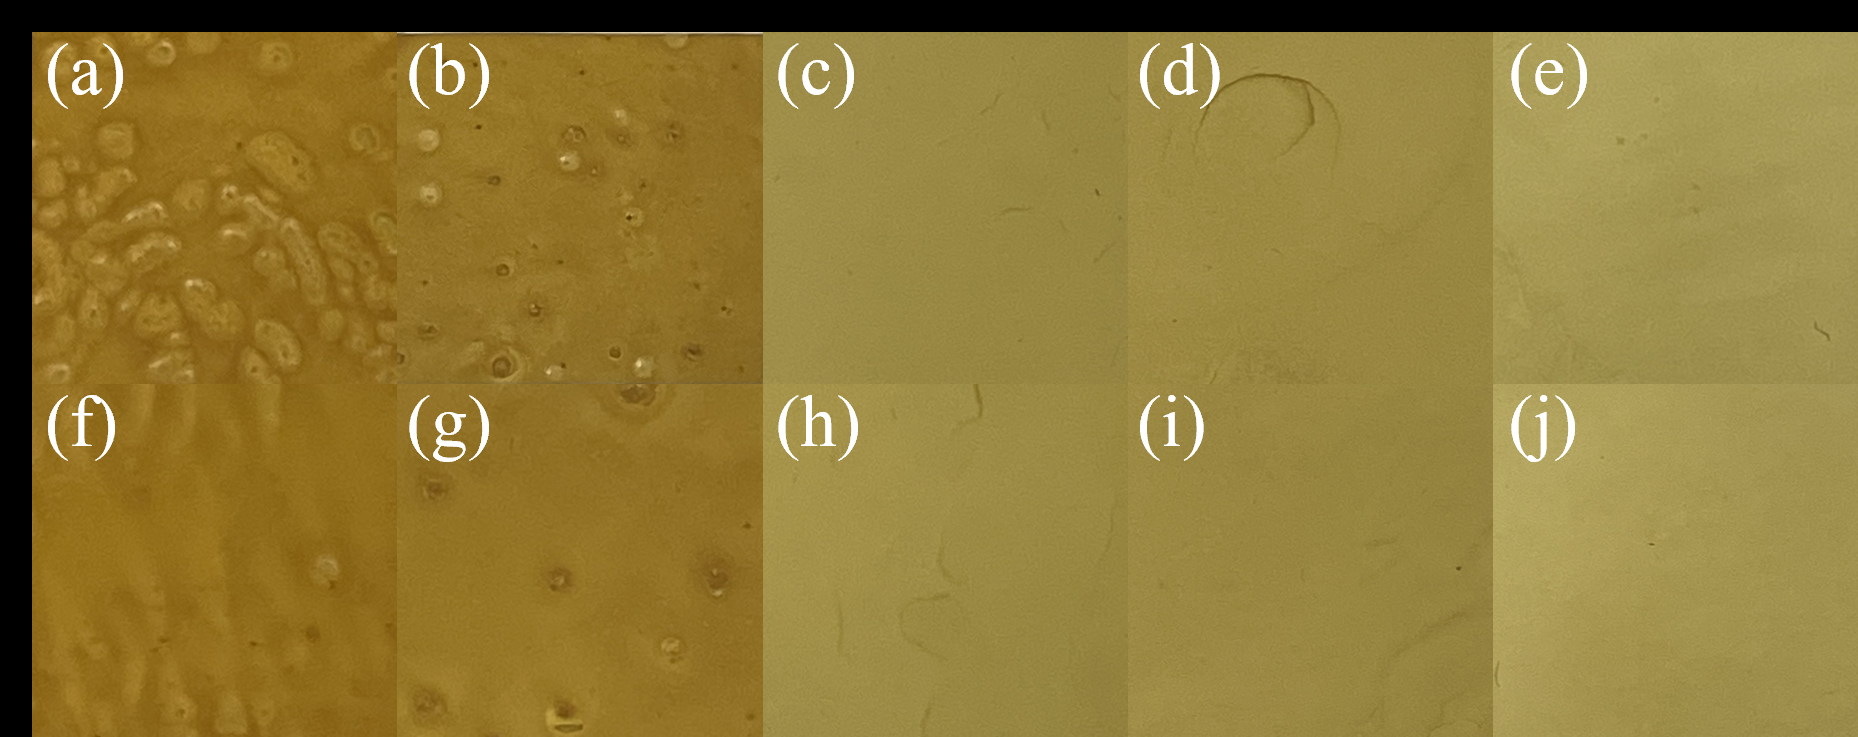
\includegraphics[width=0.9\linewidth]{FigS6_photos.png}
\caption{Photographs of the PI/h-BN films: (a--e) non-pressed and (f--j) hot-pressed at 0, 10, 30, 50, and 70~wt\% h-BN. \hl{Add composition column headers, NP/HP row labels, and a scale bar directly on the figure, and crop the black margin.}}
\label{fig:S6}
\end{figure}

\subsection{Top-view SEM}
\begin{figure}[htbp]
\centering
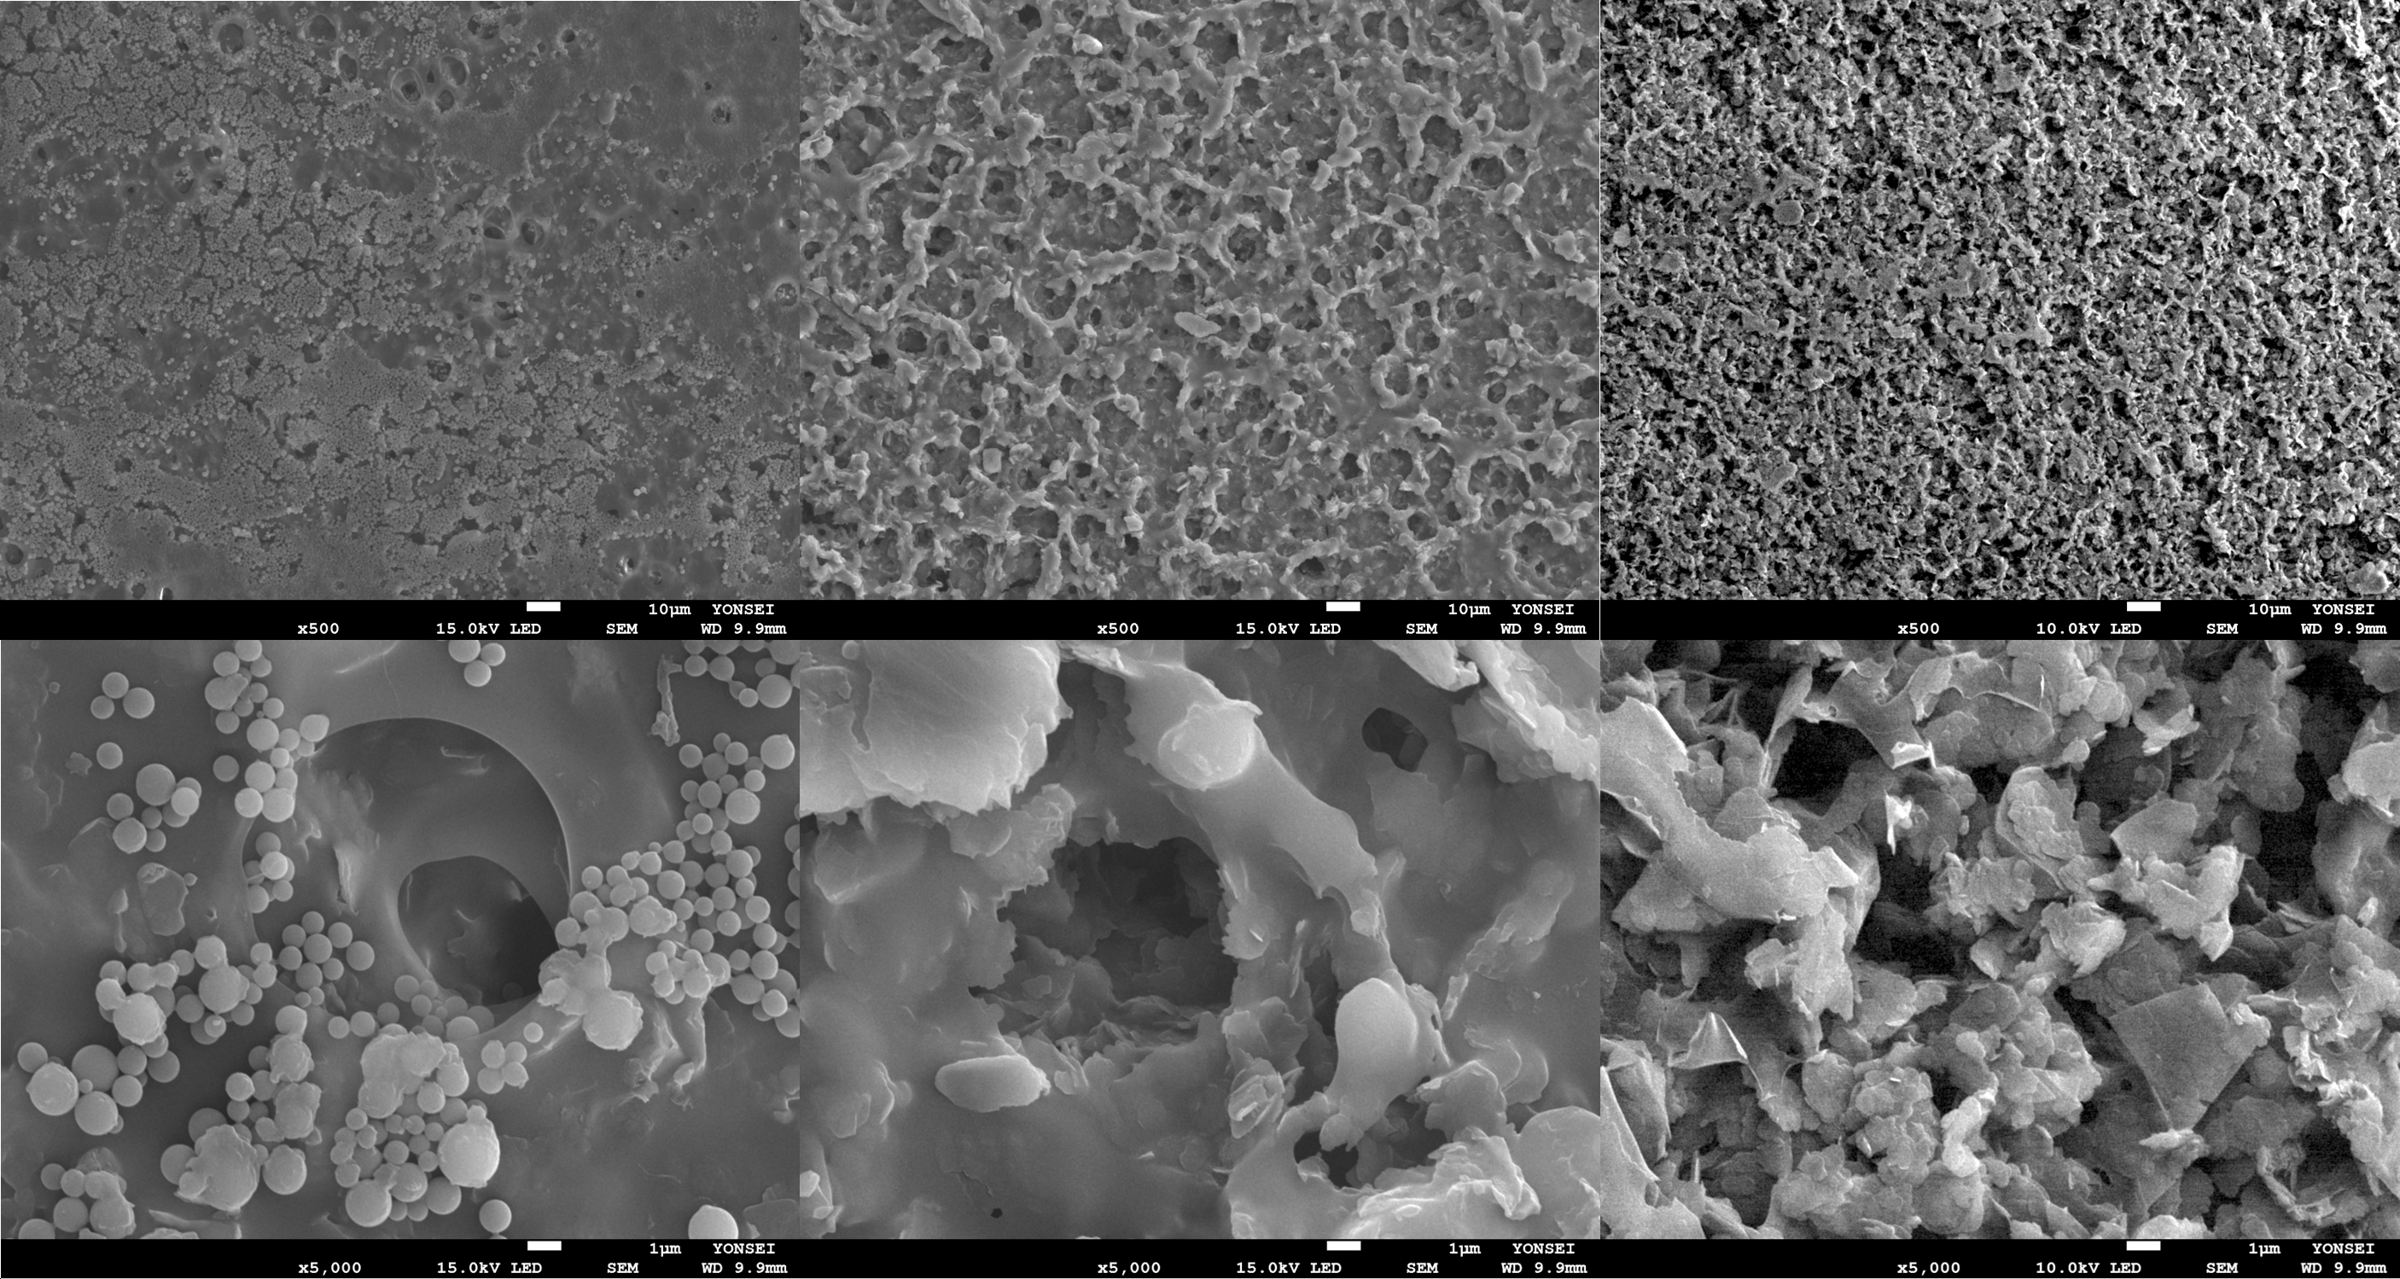
\includegraphics[width=0.9\linewidth]{FigS7_topview.png}
\caption{Top-view FE-SEM micrographs of PI/h-BN films at 30, 50, and 70~wt\% h-BN (columns) at two magnifications (rows). \hl{Label the rows by magnification ($\times$500, $\times$5{,}000) and the columns by composition on the figure.}}
\label{fig:S7}
\end{figure}

\subsection{FT-IR}
\begin{figure}[htbp]
\centering
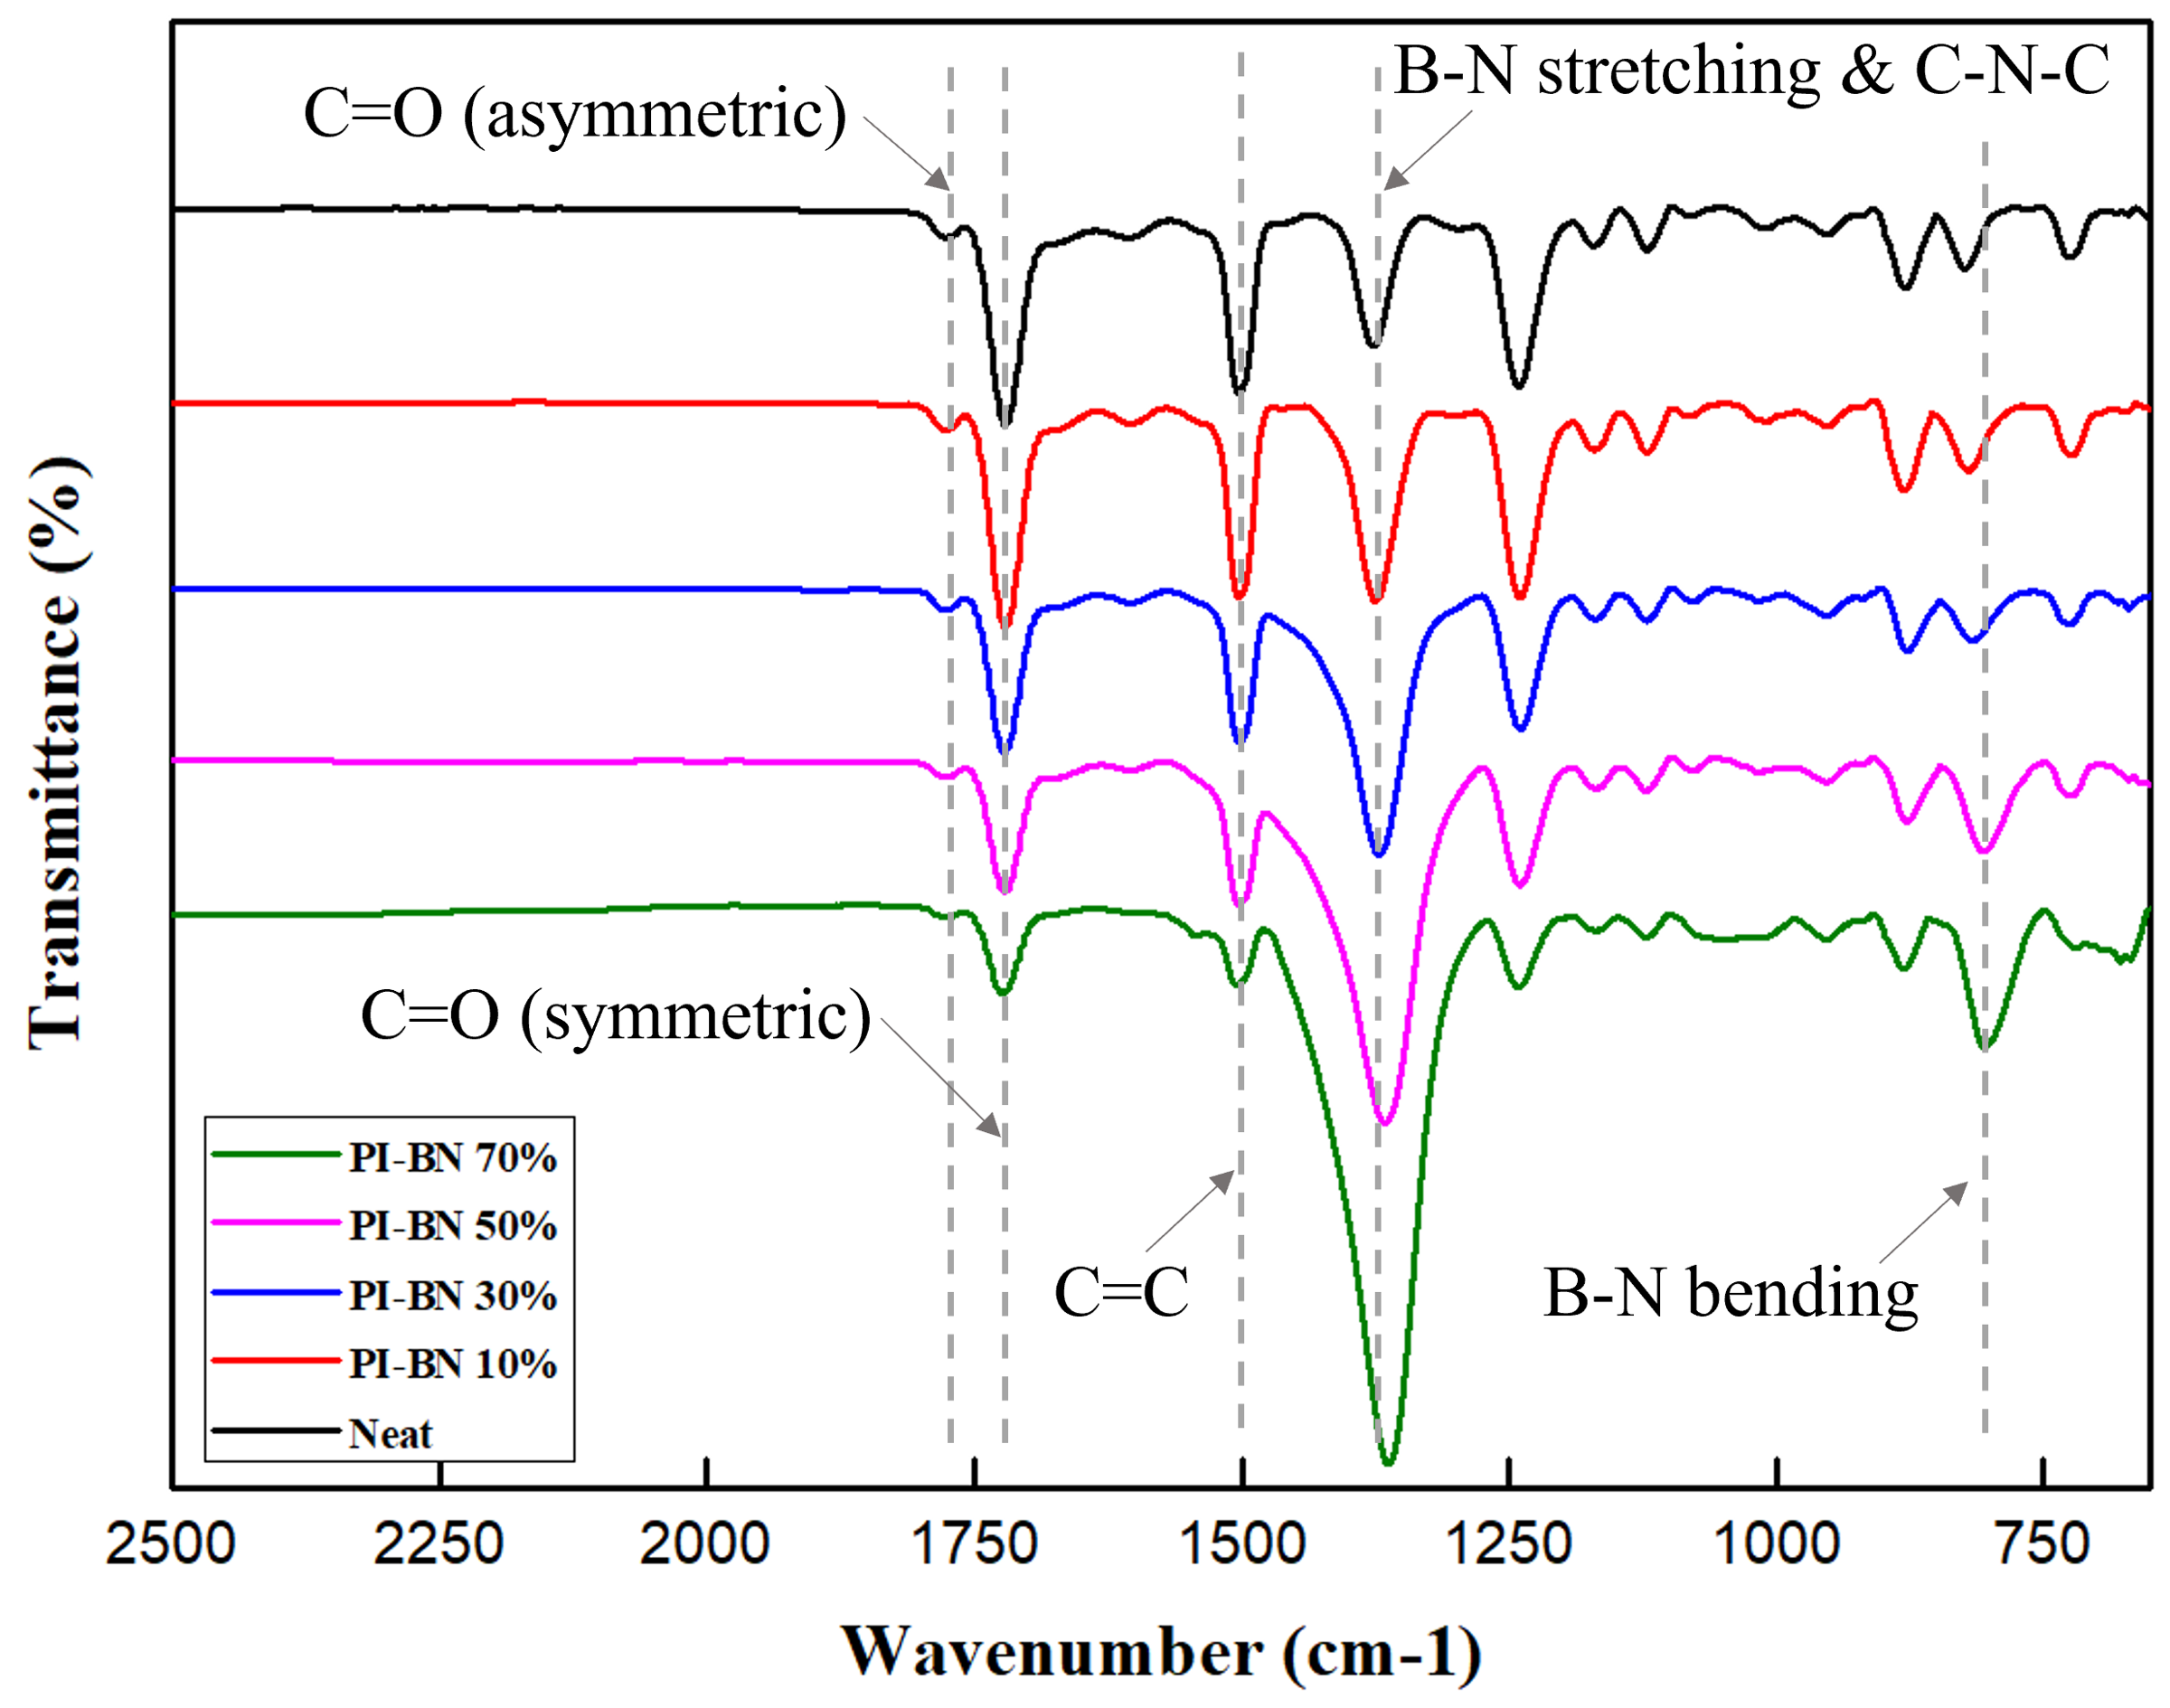
\includegraphics[width=0.75\linewidth]{FigS8_ftir.png}
\caption{FT-IR spectra (Jasco FT/IR-460 Plus, 600--\SI{4000}{\per\centi\meter}) confirming complete imidization. \hl{Confirm the band positions against the recorded spectra and use one set of values here and in Section~2.3 of the main text (currently 1720/1780 and \SI{1380}{\per\centi\meter} in the main text vs.\ 1722/1778 and \SI{1366}{\per\centi\meter} in an earlier draft of this caption). Re-plot the figure with a \si{\per\centi\meter} axis label and the typeface of the other figures.}}
\label{fig:S8}
\end{figure}

\subsection{EDS elemental analysis}
\begin{table}[htbp]
\centering
\caption{EDS elemental composition (wt\%) of PI/h-BN films (FE-SEM/EDS, JEOL-7800F). B content scales with nominal h-BN loading at $\geq$10~wt\% and is preserved upon hot-pressing.}
\label{tab:S1}
\small
\begin{tabular}{@{}lccccc@{}}
\toprule
Sample & B & C & N & O & Total \\
\midrule
NP neat     & 5.41$^{\dagger}$  & 73.72 & 3.83  & 17.04 & 100 \\
NP 10 wt\%  & 7.99  & 65.55 & 10.42 & 16.04 & 100 \\
NP 30 wt\%  & 14.70 & 54.28 & 19.36 & 11.66 & 100 \\
NP 50 wt\%  & 19.80 & 44.10 & 26.49 & 9.60  & 100 \\
NP 70 wt\%  & 29.28 & 26.65 & 38.62 & 5.45  & 100 \\
HP neat     & ---   & 75.17 & 0.00  & 24.83 & 100 \\
HP 10 wt\%  & 8.54  & 68.30 & 8.67  & 14.49 & 100 \\
HP 30 wt\%  & 14.77 & 54.74 & 18.85 & 11.64 & 100 \\
HP 50 wt\%  & 21.11 & 43.12 & 26.62 & 9.15  & 100 \\
HP 70 wt\%  & 28.17 & 29.15 & 36.48 & 6.20  & 100 \\
\bottomrule
\end{tabular}\\[3pt]
\parbox{0.85\linewidth}{\footnotesize A second NP 70~wt\% spot gave B/C/N/O = 28.81/27.93/37.01/6.25~wt\%, confirming spatial uniformity. $^{\dagger}$The apparent B signal in the neat NP film, which contains no boron, reflects the EDS quantification limit for light elements (B~K$\alpha$ overlaps the C/N/O region) and is treated as background.}
\end{table}

\hl{To be added: mercury intrusion pore-size distributions for all ten films. The comparison of open (intrusion) and total (density-derived) porosity is given in Table~3 of the main text.}

%% ------------------------------------------------------------
\section{Model details and benchmarks}
\label{si:model}

\subsection{Sequential three-phase Lewis--Nielsen formulation}
\hl{To be completed: full derivation and parameter definitions (main-text
Eqs.\ 1--3 expanded), including the step-1 (dense composite) and step-2
(pore incorporation) expressions and the packing-interaction term $\psi$.
Number the key expression as Eq.~(S8); the main text cites Eq.~S8.}

\subsection{Volume-fraction conversion}
\hl{To be completed: wt\% $\to$ vol\% conversion using $\rho_{\mathrm{PI}}
= \SI{1.42}{\gram\per\cubic\centi\meter}$ and $\rho_{\mathrm{BN}} =
\SI{2.29}{\gram\per\cubic\centi\meter}$, with the porosity-corrected film
volume fractions used throughout, and the $\rho_{\mathrm{solid}}$ values
behind the $\phi_{\mathrm{total}}$ column of Table~3 of the main text.}

\subsection{Sensitivity of the dielectric fit}
\hl{To be completed. Include a re-fit of the dielectric model using
$\phi_{\mathrm{total}}$ (density-derived) as the porosity input for the
seven films with measured density, reporting RMSE and $R^2$ side by side
with the open-porosity fit used in the main text.}

\subsection{Uncertainty propagation}
\hl{To be completed: propagation of the $\alpha$, $C_p$ and $\rho$
uncertainties into $\lam$ (about 10\%), and the uncertainty of \eps{}
including the inter-laboratory comparison of Section~4.2.}

\subsection{Benchmark against standard mixing rules}
\label{si:mixingrules}
\hl{To be completed: quantitative comparison of the calibrated LN model
against Lichtenecker, Maxwell--Garnett, and Bruggeman zero-parameter
mixing rules (the main text cites RMSE 0.26 vs.\ 0.55--0.90 over the
30--70~wt\% films; state whether NP-only or NP+HP films are included so
that the value is consistent with the NP-only RMSE of 0.25 quoted in
Section~4.2).}

%% ------------------------------------------------------------
\section{Parameter estimation protocol}
\label{si:paramest}

\subsection{Dielectric calibration}
\hl{To be completed: objective function, optimizer settings, initial
values, and convergence diagnostics.}

\subsection{Degeneracy of the unconstrained thermal fit}
\label{si:degenerate}
\hl{To be completed: demonstration that the unconstrained three-parameter
thermal fit converges to a degenerate solution ($A \to 700$, $\phimax \to
0.10$) with correlated parameters, motivating the single-parameter
calibration ($\lamBN$ fitted; $A = 5.5$, $\phimax = 0.60$ fixed). The main
text cites Section~S4.2. Include the RMSE comparison table
(constrained 0.027/0.030 vs.\ unconstrained
0.027/\SI{0.023}{\watt\per\meter\per\kelvin}); the main text references
Table~S11.}

%% ------------------------------------------------------------
\section{Python implementation}
\label{si:code}
\hl{To be completed: complete listing of the three-phase Lewis--Nielsen model
and parameter-estimation code (the Excel workbook `Model\_Calculator'
sheet implements the identical pipeline in spreadsheet form). Deposit the
code in a public repository and reference the DOI here and in the Data
availability statement.}

\end{document}
